\documentclass[11pt,a4paper,xcolor=table]{report}
\usepackage[table,xcdraw]{xcolor}
\usepackage{graphicx}
\usepackage{multirow}
\usepackage{geometry}
 \geometry{
 a4paper,
 left=25mm,
 top=20mm,
 right=20mm,
 bottom=20mm
 }
\usepackage[english]{babel}
\usepackage[T1]{fontenc}
\usepackage[utf8]{inputenc}
% Helvetica is an analogue to Arial
\usepackage{helvet}
\renewcommand{\familydefault}{\sfdefault}
\usepackage{mathptmx}
\usepackage{setspace}
\usepackage[official]{eurosym}
\usepackage{textcomp}
\usepackage{pdfpages}
\usepackage{longtable}
\usepackage{fancyhdr}
\usepackage{enumitem}
\usepackage{csquotes}
\usepackage{amsmath}
\usepackage{amsfonts}
\usepackage{caption}
\usepackage{subcaption}
\usepackage{float}
% ref packages
\usepackage{nameref}
% following  must be in this order
\usepackage{varioref}
\usepackage{hyperref}
\usepackage{cleveref}
\usepackage{algorithm}
\usepackage{algpseudocode}
\usepackage{listings}
\usepackage{xcolor}
\definecolor{codegreen}{rgb}{0,0.6,0}
\definecolor{codegray}{rgb}{0.5,0.5,0.5}
\definecolor{codepurple}{rgb}{0.58,0,0.82}
\definecolor{backcolour}{rgb}{0.95,0.95,0.92}
\lstdefinestyle{python_style}{
    backgroundcolor=\color{backcolour},   
    commentstyle=\color{codegreen},
    keywordstyle=\color{magenta},
    numberstyle=\tiny\color{codegray},
    stringstyle=\color{codepurple},
    basicstyle=\ttfamily\footnotesize,
    breakatwhitespace=false,         
    breaklines=true,                 
    captionpos=b,                    
    keepspaces=true,                 
    numbers=left,                    
    numbersep=5pt,                  
    showspaces=false,                
    showstringspaces=false,
    showtabs=false,                  
    tabsize=2
}
\lstset{style=python_style}

\usepackage[backend=biber,style=ieee]{biblatex}
\addbibresource{references.bib}

\usepackage[compact]{titlesec}
% Remove chapter headings and page break
\titleformat{\chapter}[display]
{\normalfont\Large\bfseries}{\chaptertitlename\ \thechapter}{0pt}{\Large}
\titleclass{\chapter}{straight}

% this alters "before" spacing (the second length argument) to 0
\titlespacing*{\chapter}{0pt}{0pt}{0pt}
\titlespacing*{\section}{0pt}{0pt}{0pt}
\titlespacing*{\subsection}{0pt}{0pt}{0pt}

\makeatother
% Set new lengths
\newlength{\chapheadtopskip}\setlength{\chapheadtopskip}{0pt}
\newlength{\chapheadsep}\setlength{\chapheadsep}{0pt}
\newlength{\chapheadbelowskip}\setlength{\chapheadbelowskip}{0pt}


\begin{document}

% \titleformat{\chapter}[display]
%   {\normalfont\bfseries}{}{-3em}{\Large}


\begin{titlepage}
\begin{center}


\includegraphics[width=0.8\textwidth]{assets/ntu_logo.png}

\vspace{2cm}

{\large CZ4071 Network Science}
\\[0.5cm]
{\large Assignment 2 - Final Report}

\vspace{2.5cm}

\textbf{\large Survey and Implementation of Paper: }

\vspace{0.5cm}

[7] Difan Zou, Ziniu Hu, Yewen Wang, Song Jiang, Yizhou Sun, and Quanquan Gu. “LayerDependent Importance Sampling for Training Deep and Large Graph Convolutional
Networks”. In NeurIPS 2019


\vspace{2.5cm}

Submitted by:
Team 4
\begin{table}[!htbp]
\centering
\begin{tabular}{|l|l|l|}
\hline
Eddy Lim Qing Yang & U1620115B & eddy0006@e.ntu.edu.sg \\ \hline
Shawn Kan Jung Tze& U1721495G & skan003@e.ntu.edu.sg \\ \hline
Leung Cheuk Yui & U1622880A & cleung002@e.ntu.edu.sg \\ \hline
Joshua Lim Ting Wei & U1622602G & jlim222@e.ntu.edu.sg \\ \hline
Visco Christienne Grace Regodon & U1722616L & christie001@e.ntu.edu.sg \\ \hline
Li Yuting & U1720729F & b170024@e.ntu.edu.sg \\ \hline
Nguyen Ngoc Khanh& U1720451D & C170030@e.ntu.edu.sg \\ \hline
Xing Wanting & U1721577A & wxing003@e.ntu.edu.sg \\ \hline
\end{tabular}
\end{table}

\vfill

% Bottom of the page
\bfseries SCHOOL OF COMPUTER SCIENCE AND ENGINEERING
\\
AY2019/2020 SEMESTER 2

\end{center}
\end{titlepage}

% Remove gaps from list items and list heading
\setlist[itemize]{noitemsep, topsep=-1pt}
% \doublespacing
\setlength{\parindent}{0em}
\setlength{\parskip}{1em}
\pagenumbering{arabic}
% ========================================================================

%\chapter{Background}
Graph Convolutional Networks (GCNs) applies convolution filter into graphs. Each GNC layer aggregate the embeddings of a node's neighbours from the previous layer and transforms it in a non-lineary fashion to obtain the new contextualised node representation \cite{assigned_paper_zou2019layer}. Through stacking multiple GCN layers, each node representation is thus able to make use of a wide receptive field from both immediate and distant node neighbours, which intuitively increases model capacity \cite{assigned_paper_zou2019layer}.

\chapter{Problem Statement}
GCNs are rising in popularity due to favourable implementations in various areas. However, training GCNs is difficult in practice due to the fact that graph data can be extremely large, unlike tokens in a paragraph or pixels in an image that normally have a fixed size. A node's embedding in GCNs depend recursively on all its neighbours' embeddings, causing an exponential growth in computation dependency depending on the number of layers. Thus, GCNs are still inapplicable in large-scale graphs.

Classical solutions to the size problem includes sampling-based methods such as the "node-wise neighbour-sampling" and "layer-wise importance sampling" that train GCNs on a subset of nodes. The "node-wise neighbour-sampling", which recursively samples a fixed number of neighbour nodes and calculates each node's embedding \cite{assigned_paper_zou2019layer}. However, when nodes share the same sampled neighbour, the neighbour's embedding has to be reevaluated and the redundancy increases exponentially with more layers. This results in an exponentially increasing computation cost with a node's neighbour size.

An the other hand, the "layer-wise importance sampling" calculates the sampling probability based on the node's degree and a fixed number of nodes is sampled for each layer. The sampled nodes are used to build a smaller, now sampled adjacency matrix, which reduces computation costs. A problem, however, is that sampled nodes from adjacent layers may not be connected due to the fact that sampling probability is independent for each layer. This may cause the matrix to be extremely sparse and so, the sampled nodes may suffer from sparse connectivity problems.

Due to the limitations of the classical methods, alternative methods such as the VR-GCN \cite{chen2017stochastic}, FastGCN \cite{chen2018fastgcn} and Cluster-GCN \cite{chiang2019cluster} have been proposed in the recent years. The FastGCN reduces the computation cost by using only sampled nodes to build a sampled adjacency matrix \cite{chen2018fastgcn}, while the VR-GCN uses variance
reduction techniques to improve sample complexity to reduce computation redundancy \cite{chen2017stochastic} and the Cluster-GCN does preprocessing before training the GCN by restricting the sampled neighbors within some dense subgraphs through a graph clustering algorithm \cite{chiang2019cluster}. However, it is argued in \cite{assigned_paper_zou2019layer} that those proposed methods still cannot resolve the issue of redundant
computations completely.


% \chapter{Related Works}
Sample cite \cite{gunther2010neuralnet}.
% \input{mid-progress_report/solution}
\chapter{Real-World Applications}
Due to its flexibility, GCNs can be applied in various domains in the real-world. Examples of such domains are in the application of GCNs in Computer Vision (CV), Natural Language Processing (NLP) and other sciences.

CV has been a hot research area in the past decades. Although classic convolutional neural networks (CNN) have achieved great successes in CV, it is not feasible to encode the intrinsic graph structures in the specific learning tasks. On the other hand, GCNs have been applied and achieved a comparable or even better performance in some CV problems. For example, \cite{cui2018context} proposes a graph CNN to leverage both the semantic graphs of words and spatial scene graph for visual relationship detection. Furthermore, in \cite{chen2017photographic}, it is shown that a GCN model can be used to process the input scene graph and generate the images by a cascaded refinement network for photographic image synthesis. Moreover, GCNs can also be applied in videos. \cite{yan2018spatial} applied GCN to perform action recognition by proposing a spatial-temporal graph convolutional model to eliminate the need of hand-crafted part assignment which achieved a greater expressive power.

GCNs also have applications in NLP. For text classification, citation network can be constructed with the documents as nodes and the citation relationships among them as edges. And node classification can be a straightforward way to classify documents into different categories. In \cite{yao2019graph}, TextGCN performs text classification by modeling a whole corpus to a heterogeneous graph and learn word embedding and document embedding simultaneously, followed by a softmax classifier for text classification. In addition, a syntactic GCN model is developed and it can be used on top of syntactic dependence trees, which is suitable for semantic role labelling \cite{marcheggiani2017encoding} and neural machine translation \cite{bastings2017graph}.

GCNs are also applied in other domains outside of Computer Science.

In chemistry, \cite{zitnik2018modeling} first models drug-protein target interactions and protein-protein interactions into a multimodal graph, and then graph convolutions is applied to predict polypharmacy side effects. 

In material science, \cite{xie2018crystal} proposes a crystal GCN to directly learn material properties from the connections of atoms in the crystal. 

In social sciences, GCNs have been widely used for social recommendation to improve the recommendation performances based on user-item interactions and/or user-user interactions. \cite{wu2019neural} proposes a neural influence diffusion model for better social recommendation by considering the influence of trusted friends.

% \chapter{Conclusion}

The difference between Layer-Dependent Importance Sampling (LADIES) method and the Full-Batch sampling method is that the LADIES method does not sample the whole graph. It samples the important nodes that will be processed in the neural network. However, the Full-Batch sampling method uses the whole graph as training samples. The methods can be considered as batch gradient descent and stochastic gradient descent. Throughout the experiments, it is found that Full-Batch sampling has a better execution time as compared to LADIES sampling. However, due to space complexity, Full-Batch sampling cannot be scaled up for large-size data. On the other hand, by the nature of stochastic gradient descent, LADIES method takes the advantage of conducting many updates in a batch of data, it converges faster than Full-Batch sampling.

\chapter{Further Research}

It has been observed that the execution time of LADIES method is at least 1.5 times slower than Full-Batch method caused by the inefficiency in sparse matrix implementation. A better implementation is possible to yield better results.

\newpage
\pagenumbering{roman}
% %%%% ADD BIBLOGARPHY
\printbibliography
 \chapter{Introduction}
Graph Convolutional Networks (GCNs) applies convolution filter into graphs. Each GNC layer aggregate the embeddings of a node's neighbours from the previous layer and transforms it in a non-lineary fashion to obtain the new contextualised node representation. Through stacking multiple GCN layers, each node representation is thus able to make use of a wide receptive field from both immediate and distant node neighbours, which intuitively increases model capacity \cite{assigned_paper_zou2019layer}. 

An experiment will be conducted in relation to the paper in \cite{assigned_paper_zou2019layer}. The experiment will include the implementation and adaptation of algorithms developed from the paper and the replication of experimental results from the algorithms implemented in the paper.

\chapter{Background}

\section{Problem Statement and Related Works}
GCNs are rising in popularity due to favourable implementations in various areas. However, training GCNs is difficult in practice due to the fact that graph data can be extremely large, unlike tokens in a paragraph or pixels in an image that normally have a fixed size. A node's embedding in GCNs depend recursively on all its neighbours' embeddings, causing an exponential growth in computation dependency depending on the number of layers. Thus, GCNs are still inapplicable in large-scale graphs.

Classical solutions to the size problem includes sampling-based methods such as the "node-wise neighbour-sampling" and "layer-wise importance sampling" that train GCNs on a subset of nodes. The "node-wise neighbour-sampling", which recursively samples a fixed number of neighbour nodes and calculates each node's embedding \cite{assigned_paper_zou2019layer}. However, when nodes share the same sampled neighbour, the neighbour's embedding has to be reevaluated and the redundancy increases exponentially with more layers. This results in an exponentially increasing computation cost with a node's neighbour size.

An the other hand, the "layer-wise importance sampling" calculates the sampling probability based on the node's degree and a fixed number of nodes is sampled for each layer. The sampled nodes are used to build a smaller, now sampled adjacency matrix, which reduces computation costs. A problem, however, is that sampled nodes from adjacent layers may not be connected due to the fact that sampling probability is independent for each layer. This may cause the matrix to be extremely sparse and so, the sampled nodes may suffer from sparse connectivity problems.

Due to the limitations of the classical methods, alternative methods such as the VR-GCN \cite{chen2017stochastic}, FastGCN \cite{chen2018fastgcn} and Cluster-GCN \cite{chiang2019cluster} have been proposed in the recent years. The FastGCN reduces the computation cost by using only sampled nodes to build a sampled adjacency matrix \cite{chen2018fastgcn}, while the VR-GCN uses variance
reduction techniques to improve sample complexity to reduce computation redundancy \cite{chen2017stochastic} and the Cluster-GCN does preprocessing before training the GCN by restricting the sampled neighbors within some dense subgraphs through a graph clustering algorithm \cite{chiang2019cluster}. However, it is argued in \cite{assigned_paper_zou2019layer} that those proposed methods still cannot resolve the issue of redundant
computations completely.


\section{Real-World Applications}
Due to its flexibility, GCNs can be applied in various domains in the real-world. Examples of such domains are in the application of GCNs in Computer Vision (CV), Natural Language Processing (NLP) and other sciences.

CV has been a hot research area in the past decades. Although classic convolutional neural networks (CNN) have achieved great successes in CV, it is not feasible to encode the intrinsic graph structures in the specific learning tasks. On the other hand, GCNs have been applied and achieved a comparable or even better performance in some CV problems. For example, \cite{cui2018context} proposes a graph CNN to leverage both the semantic graphs of words and spatial scene graph for visual relationship detection. Furthermore, in \cite{chen2017photographic}, it is shown that a GCN model can be used to process the input scene graph and generate the images by a cascaded refinement network for photographic image synthesis. Moreover, GCNs can also be applied in videos. \cite{yan2018spatial} applied GCN to perform action recognition by proposing a spatial-temporal graph convolutional model to eliminate the need of hand-crafted part assignment which achieved a greater expressive power.

GCNs also have applications in NLP. For text classification, citation network can be constructed with the documents as nodes and the citation relationships among them as edges. And node classification can be a straightforward way to classify documents into different categories. In \cite{yao2019graph}, TextGCN performs text classification by modeling a whole corpus to a heterogeneous graph and learn word embedding and document embedding simultaneously, followed by a softmax classifier for text classification. In addition, a syntactic GCN model is developed and it can be used on top of syntactic dependence trees, which is suitable for semantic role labelling \cite{marcheggiani2017encoding} and neural machine translation \cite{bastings2017graph}.

GCNs are also applied in other domains outside of Computer Science.

In chemistry, \cite{zitnik2018modeling} first models drug-protein target interactions and protein-protein interactions into a multimodal graph, and then graph convolutions is applied to predict polypharmacy side effects. 

In material science, \cite{xie2018crystal} proposes a crystal GCN to directly learn material properties from the connections of atoms in the crystal. 

In social sciences, GCNs have been widely used for social recommendation to improve the recommendation performances based on user-item interactions and/or user-user interactions. \cite{wu2019neural} proposes a neural influence diffusion model for better social recommendation by considering the influence of trusted friends.


\chapter{The Challenges of the Problem}

The goal of the LADIES sampling method is to improve on the previously implemented sampling methods. The issue with the other methods is that it requires high computation and memory cost. The weakness of node-wise neighbour-sampling method is that it recursively samples a fixed number of neighbours which leads to high computation cost. Furthermore, layer-wise importance-sampling method discards the neighbour-dependent constraints and thus the nodes sampled will lead to high memory cost. 

A good sampling method should satisfy 2 criteria. The sampling method has to be layer-wise, neighbour-dependent and must use importance-sampling. The LADIES sampling method solves these issues by mini-batch processing. Every iteration, it chooses a mini-batch nodes then dependent-sampling of neighbours is applied with a fixed size of sampled nodes that limits the space complexity.
\chapter{Experiment}
Our initialization for table assignment was chosen such at each customer is at a separate table at the beginning. Louvain method \cite{blondel2008fast} was used in MCLA algorithm due to its low time complexity.
\section{Synthetic Networks}

\subsection{Setup}

In this section, the performance of proposed method is demonstrated using synthetic network as described below:

\begin{algorithm}[H]
\label{alg:powerlaw}
\caption{Power-Law clustering generator}
\textbf{Input:}\\
    $\gamma$: gamma constant \\
    $K$: number of clusters\\

\textbf{Output:}\\
    $size$: relative sizes of clusters distributed according to density $f(x) \propto x^{-\gamma}$\\
    
\begin{algorithmic}

\State $size = \{\frac{k - 0.5}{K}\}_{k=1}^{K}$

\State $size = size^\frac{1}{1 - \gamma}$ \Comment{Element-wise operation}

\State $size = \frac{size}{size.sum()}$ \Comment{Element-wise operation}

\end{algorithmic}
\end{algorithm}

Stochastic Block Model is used to generate the networks with power-law cluster sizes, average degree and intra-cluster edge probability over inter-cluster edge probability $p_{in} / p_{out} = 10$.

We performed grid search over the set of parameters as follow: Number of vertices $|V| \in \{500, 1000, 1500, 2000\}$, average degree $avgdeg \in \{10, 20, 30, 40, 50\}$, scale parameter $s \in \{1000, 2000, ..., 29000\}$

The same node embedding from \emph{Deepwalk} was used for different scale parameter. We fixed these parameters: $\gamma = 2.5$, embedding dimension $d=50$, walks per vertex $\gamma = 2|E|/|V|$, context size $c = 5$, walk length $l = 3c$, receptive field hop $h=1$, \emph{Deepwalk} epochs = 10 and \emph{ddCRP} epochs = 10 for each run. We took only the last 5 iterations from \emph{ddCRP} as the set of stable states.

We compared two versions: initialized Kmeans using ddCRP and MCLA \textbf{ddcrp-mcla} and initialized Kmeans "k-means++" \textbf{kmeans++} with 10 times of initialization which is builtin within sklearn library.

\subsection{Results}
\subsubsection{Modularity}

\begin{figure}
    \centering
    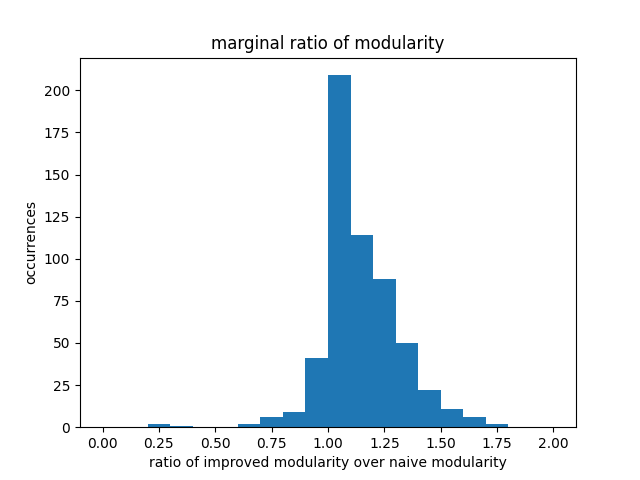
\includegraphics[width=0.8\textwidth]{report/assets/results/ratio.png}
    \caption{Distribution of ratio $\frac{\text{modularity(ddcrp-mcla)}}{\text{modularity(kmeans++)}}$}
    \label{fig:ratio}
\end{figure}


Modularity of each algorithm was evaluated for each setup. Figure \ref{fig:ratio} represent the distribution of the ratio $\frac{\text{modularity(ddcrp-mcla)}}{\text{modularity(kmeans++)}}$. The figure reflects the superior performance of \textbf{ddcrp-mcla} initialization for kmeans as compare to \textbf{kmeans++}. On average, \textbf{ddcrp-mcla} performs better than \textbf{kmeans++} by 14.1\% with a standard deviation of 17.5\%.

Figure \ref{fig:modularity10}, \ref{fig:modularity20}, \ref{fig:modularity30}, \ref{fig:modularity40}, and \ref{fig:modularity50} show that the modularity obtained by \textbf{ddcrp-mcla} always better than \textbf{kmeans++} on all different predicted number of clusters even if the estimation diverges from the true number of clusters (50).

\begin{figure}
    \centering
    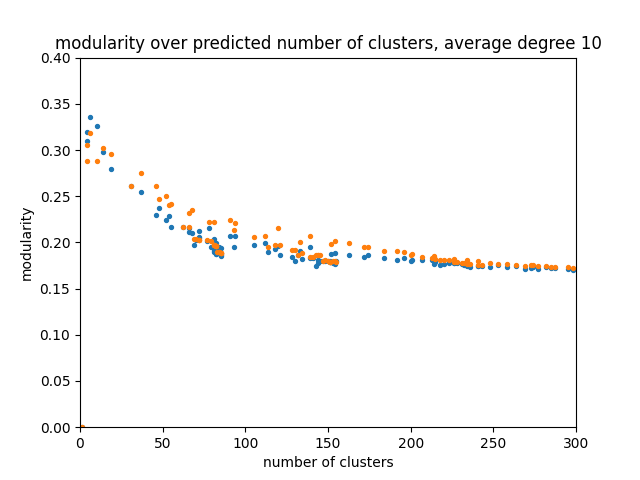
\includegraphics[width=0.8\textwidth]{report/assets/results/modularity10.png}
    \caption{Modularity w.r.t predicted number of clusters for average degree 10 (\textbf{ddcrp-mcla}: orange, \textbf{kmeans++}: blue)}
    \label{fig:modularity10}
\end{figure}

\begin{figure}
    \centering
    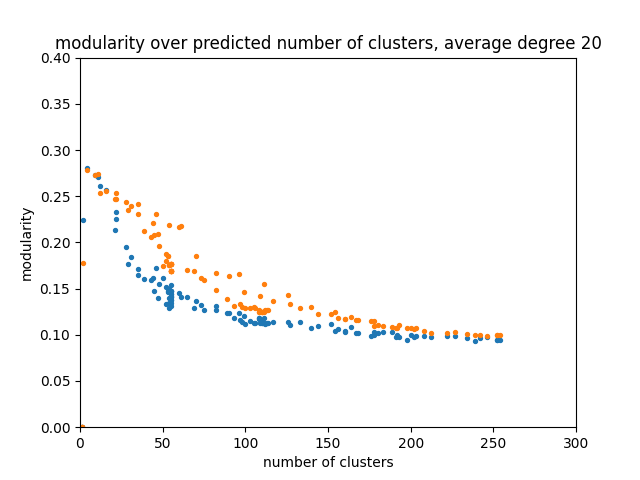
\includegraphics[width=0.8\textwidth]{report/assets/results/modularity20.png}
    \caption{Modularity w.r.t predicted number of clusters for average degree 20 (\textbf{ddcrp-mcla}: orange, \textbf{kmeans++}: blue)}
    \label{fig:modularity20}
\end{figure}

\begin{figure}
    \centering
    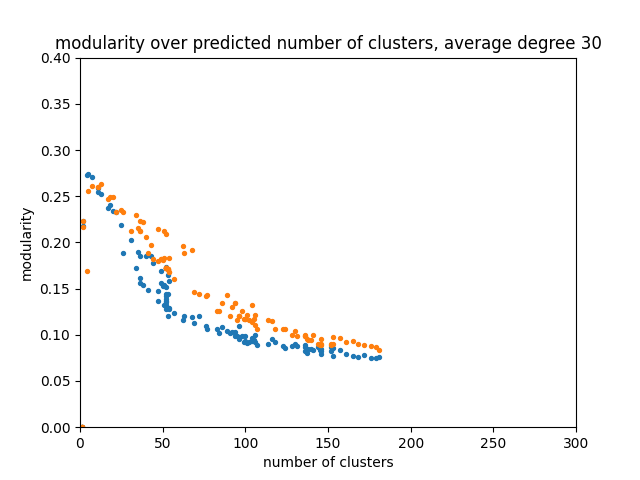
\includegraphics[width=0.8\textwidth]{report/assets/results/modularity30.png}
    \caption{Modularity w.r.t predicted number of clusters for average degree 30 (\textbf{ddcrp-mcla}: orange, \textbf{kmeans++}: blue)}
    \label{fig:modularity30}
\end{figure}

\begin{figure}
    \centering
    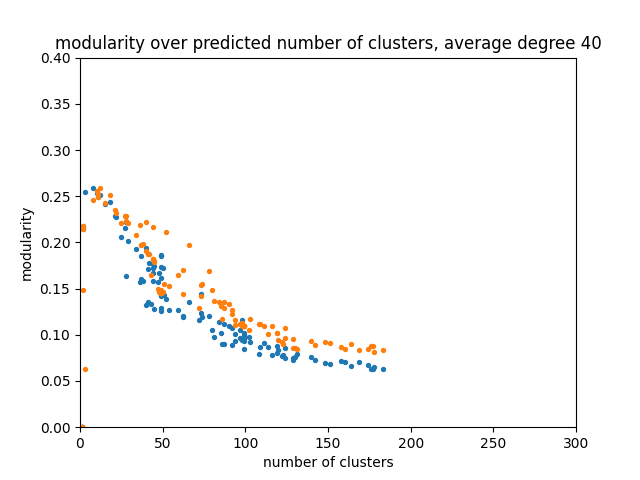
\includegraphics[width=0.8\textwidth]{report/assets/results/modularity40.png}
    \caption{Modularity w.r.t predicted number of clusters for average degree 40 (\textbf{ddcrp-mcla}: orange, \textbf{kmeans++}: blue)}
    \label{fig:modularity40}
\end{figure}

\begin{figure}
    \centering
    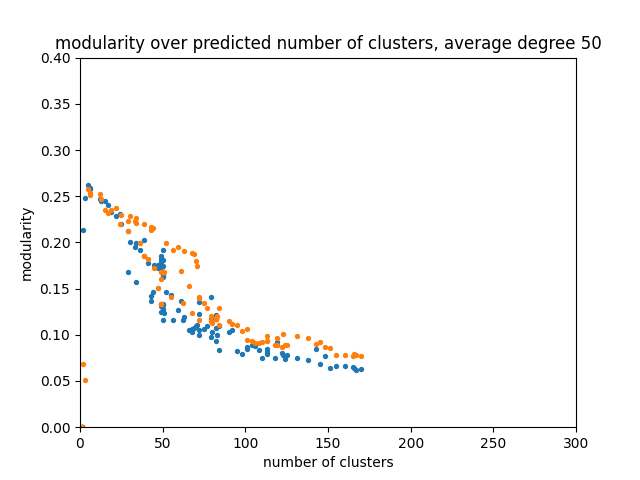
\includegraphics[width=0.8\textwidth]{report/assets/results/modularity50.png}
    \caption{Modularity w.r.t predicted number of clusters for average degree 50 (\textbf{ddcrp-mcla}: orange, \textbf{kmeans++}: blue)}
    \label{fig:modularity50}
\end{figure}

The ratio $\frac{\text{modularity(ddcrp-mcla)}}{\text{modularity(kmeans++)}}$ depends on its predicted number of clusters as shown in figure \ref{fig:ratio_cluster}. The ratio appears to achieve its best performance at the predicted number of clusters between 50 and 100 where the actual number of clusters is 50.

\begin{figure}
    \centering
    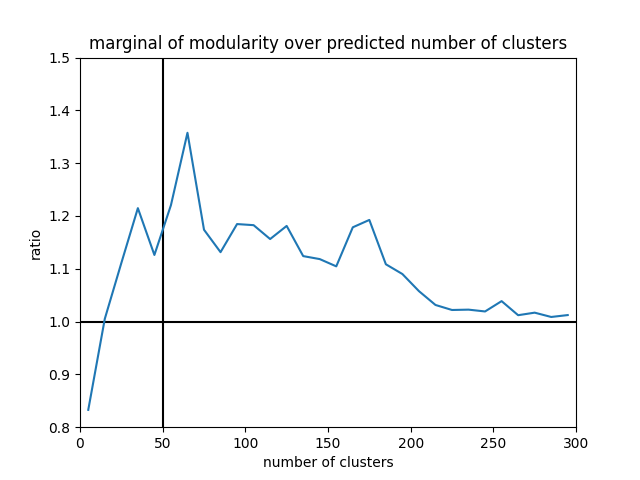
\includegraphics[width=0.8\textwidth]{report/assets/results/ratio_cluster.png}
    \caption{ratio $\frac{\text{modularity(ddcrp-mcla)}}{\text{modularity(kmeans++)}}$ over predicted number of clusters}
    \label{fig:ratio_cluster}
\end{figure}

\section{Real Networks}

\subsection{Setup}

In this experiment, we used the dataset at \cite{paranjape2017motifs}. The temporal network consists of 986 nodes and 332334 temporal edges in the time span of 803 days. We firstly sorted the temporal edges by its timestamp. Then we splitted the set of temporal edges into 1000 equal folds where each fold has roughly 332 edges. We set the window size of 10 folds. After each iteration, we slided the window by 1 fold. We then took the two edge timestamps of the window and filtered all the temporal edges between these timestamps as the set of edges for the graph snapshot.

Similar to the previous experiment, we set embedding dimension $d=50$, walks per vertex $\gamma = 2|E|/|V|$, context size $c = 5$, walk length $l = 3c$, \emph{Deepwalk} epochs = 10 and \emph{ddCRP} epochs = 10 for each run. We took only the last 5 iterations from \emph{ddCRP} as the set of stable states.

We performed grid search over the set of parameters as follow. Receptive field hop $h \in \{1, 2\}$, scale parameter $s \in \{1000, 2000, ..., 8000\}$

\subsection{Results}
\subsubsection{Modularity}
Figure \ref{fig:ratio_cluster_real} shows the ratio between $\frac{\text{modularity(ddcrp-mcla)}}{\text{modularity(kmeans++)}}$ over different predicted number of clusters. If we limit the predicted number of clusters to be greater than 60, the \textbf{ddcrp-mcla} method performs better than \textbf{kmeans++} by 4.4\% with a standard deviation of 5.6\%.

\begin{figure}
    \centering
    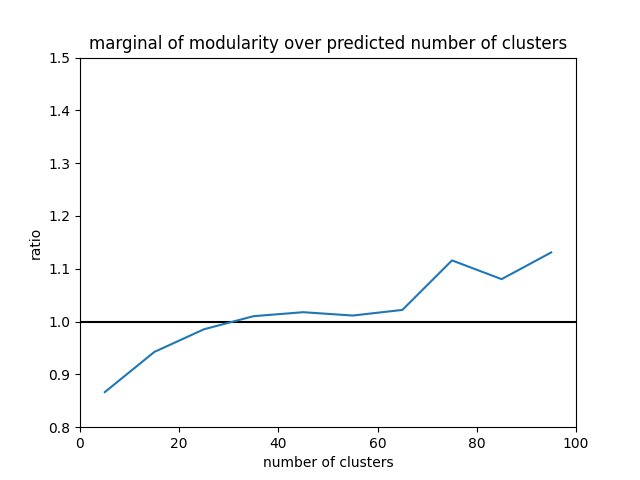
\includegraphics[width=0.8\textwidth]{report/assets/results/ratio_cluster_real.png}
    \caption{ratio $\frac{\text{modularity(ddcrp-mcla)}}{\text{modularity(kmeans++)}}$ over predicted number of clusters}
    \label{fig:ratio_cluster_real}
\end{figure}

\subsubsection{Clustering Evolution}

Our \emph{MCLA} algorithm is capable to produce some useful response from the evolution of clustering. Noted that, these results are completely automated. Textbox \ref{textbox:message}.

\fbox{\begin{minipage}{15em}
message type: join

	9 nodes remained
	
	3 nodes joined
	
	0 nodes left
	
message type: old

	2 nodes remained
	
	0 nodes joined
	
	0 nodes left
	
message type: old

	0 nodes remained
	
	25 nodes joined
	
	7 nodes left
	
message type: old

	3 nodes remained
	
	0 nodes joined
	
	0 nodes left
	
message type: join

	418 nodes remained
	
	0 nodes joined
	
	153 nodes left
	
	...
\label{textbox:message}
\end{minipage}}
\chapter{Conclusion}

The difference between Layer-Dependent Importance Sampling (LADIES) method and the Full-Batch sampling method is that the LADIES method does not sample the whole graph. It samples the important nodes that will be processed in the neural network. However, the Full-Batch sampling method uses the whole graph as training samples. The methods can be considered as batch gradient descent and stochastic gradient descent. Throughout the experiments, it is found that Full-Batch sampling has a better execution time as compared to LADIES sampling. However, due to space complexity, Full-Batch sampling cannot be scaled up for large-size data. On the other hand, by the nature of stochastic gradient descent, LADIES method takes the advantage of conducting many updates in a batch of data, it converges faster than Full-Batch sampling.

\chapter{Further Research}

It has been observed that the execution time of LADIES method is at least 1.5 times slower than Full-Batch method caused by the inefficiency in sparse matrix implementation. A better implementation is possible to yield better results.

\newpage
\pagenumbering{roman}
% %%%% ADD BIBLOGARPHY
\printbibliography

\newpage
\pagenumbering{roman}
\newpage
\appendix
\chapter{Experiment Code}
\begin{lstlisting}[language=Python, caption= Training code, label=ls:train_code]
import pdb
import argparse
from typing import List, Dict
from types import SimpleNamespace
import multiprocessing as mp
import time

import numpy as np
import scipy as sp
import torch
import torch.nn as nn
import torch.nn.functional as F
import torch.optim as optim
from sklearn.metrics import f1_score
from sklearn.linear_model import LinearRegression
from torchviz import make_dot

from module import GCN, GCNLinear
from load_data import load_random_block
from sampler import full_sampler, ladies_sampler
from utils import adj_to_lap_matrix, row_normalize, sparse_mx_to_torch_sparse_tensor, sparse_fill


#np.seterr(all="raise")

def random_sampling_train(args: SimpleNamespace, model: SimpleNamespace, data: SimpleNamespace) -> SimpleNamespace:
  if args.batch_size <= 0 or args.batch_size >= len(data.train_nodes):
    batch_nodes = data.train_nodes
  else:
    batch_nodes = np.random.choice(data.train_nodes, size= args.batch_size, replace= True)
  sample = model.sampler(
    batch_nodes= batch_nodes,
    samp_num_list= [len(batch_nodes) for _ in range(args.num_layers)],
    num_nodes= data.num_nodes,
    lap_matrix= data.lap_matrix,
    lap2_matrix= data.lap2_matrix,
    num_layers= args.num_layers,
  )
  return sample

def sampling_valid(args: SimpleNamespace, model: SimpleNamespace, data: SimpleNamespace) -> SimpleNamespace:
  sample = full_sampler(
    #batch_nodes= data.valid_nodes,
    batch_nodes= np.arange(data.num_nodes),
    samp_num_list= None,
    num_nodes= data.num_nodes,
    lap_matrix= data.lap_matrix,
    lap2_matrix= None,
    num_layers= args.num_layers,
  )
  return sample



if __name__ == "__main__":
  # load args
  parser = argparse.ArgumentParser(description='Training GCN')
  parser.add_argument('--hidden_features', type=int, default=64,
                      help='hidden layer embedding dimension')
  parser.add_argument('--num_epochs', type=int, default= 10,
                      help='Number of epochs')
  parser.add_argument('--batch_size', type=int, default=64,
                      help='batch_size: number of sampled nodes at output layer')
  parser.add_argument('--num_layers', type=int, default=5,
                      help='Number of GCN layers')
  parser.add_argument('--sampling_method', type=str, default='full',
                      help='sampling algorithms: full/ladies')
  parser.add_argument('--cuda', type=int, default=-1,
                      help='GPU ID, (-1) for CPU')
  parser.add_argument('--dropout', type=float, default= 0.5,
                    help='dropout probability')
  parser.add_argument('--learning_rate', type=float, default= 1e-3,
                    help='learning rate')
  parser.add_argument('--num_nodes', type=int, default=100,
                      help='number of network nodes in random block model')

  args = parser.parse_args()
  print(args)
  # set up device
  if args.cuda != -1:
    device = torch.device("cuda:" + str(args.cuda))
  else:
    device = torch.device("cpu")
  # load data
  all = args.num_nodes
  half = int(all/2)
  p1 = np.log(all) / all
  p2 = p1 / all
  data = load_random_block(
    [half, all-half],
    [[p1, p2], [p2, p1]],
  )
  data.num_nodes = data.features.shape[0]
  data.in_features = data.features.shape[1]
  data.out_features = len(np.unique(data.labels))
  data.lap_matrix = row_normalize(adj_to_lap_matrix(data.adj_matrix))
  data.lap2_matrix = data.lap_matrix.multiply(data.lap_matrix)

  if args.sampling_method == "full":
    args.batch_size = len(data.train_nodes)
  # create pool
  pool = mp.Pool(processes= 1)
  # create model
  model: SimpleNamespace = SimpleNamespace()
  model.sampler = full_sampler
  if args.sampling_method == "ladies":
    model.sampler = ladies_sampler
  model.module = GCNLinear(
    encoder= GCN(
      in_features= data.in_features,
      hidden_features= args.hidden_features,
      out_features= args.hidden_features,
      num_layers= args.num_layers,
      dropout= args.dropout
    ),
    in_features= args.hidden_features,
    out_features= data.out_features,
    dropout= args.dropout,
  )


  model.module.to(device)
  optimizer = optim.Adam(filter(lambda p: p.requires_grad, model.module.parameters()), lr=args.learning_rate)
  criterion = nn.CrossEntropyLoss()
  times = []
  losses = []
  f1s = []
  next_sample_async = None
  sample = None

  #START TRAINING
  start = time.time()
  try:
    for epoch in range(args.num_epochs):
      # train
      model.module.train() # train mode
      print(f"Epoch {epoch}: ", flush= True)
      num_iterations = int(data.num_nodes / args.batch_size)
      for iter in range(num_iterations):
        print(f"\tIteration {iter}: ", end= "", flush= True)
        if next_sample_async is None:
          sample = random_sampling_train(args, model, data)
        else:
          sample = next_sample_async.get()
        next_sample_async = pool.apply_async(random_sampling_train, args= (args, model, data))
        optimizer.zero_grad()
        
        output = model.module(
          x= sparse_mx_to_torch_sparse_tensor(sparse_fill(shape= data.features.shape, mx= data.features[sample.input_nodes], row= sample.input_nodes)),
          adjs= list(map(lambda adj: sparse_mx_to_torch_sparse_tensor(adj).to(device), sample.adjs)),
        )

        loss = criterion(
          output[sample.output_nodes],
          torch.from_numpy(data.labels[sample.output_nodes]).long(),
        )
        loss.backward()
        torch.nn.utils.clip_grad_norm_(model.module.parameters(), 0.2)
        optimizer.step()


        #if epoch == 0 and iter == 0:
        #  dot = make_dot(loss.mean(), params= dict(model.module.named_parameters()))
        #  dot.render("test.gv", view= True)

        loss = loss.detach().cpu()
        print(f"Loss {loss}", flush= True)
      # eval
      model.module.eval() # eval mode
      sample = sampling_valid(args, model, data)
      output = model.module(
        x= sparse_mx_to_torch_sparse_tensor(data.features[sample.input_nodes]),
        adjs= list(map(lambda adj: sparse_mx_to_torch_sparse_tensor(adj).to(device), sample.adjs)),
      )
      loss = criterion(
        output[sample.output_nodes],
        torch.from_numpy(data.labels[sample.output_nodes]).long(),
      )
      
      output = output.detach().cpu()
      loss = loss.detach().cpu()
      f1 = f1_score(
        output[sample.output_nodes].argmax(dim=1),
        data.labels[sample.output_nodes],
        average= "micro",
      )
      times.append(time.time() - start)
      losses.append(loss)
      f1s.append(f1)

      epochs = np.arange(len(times)).reshape(-1, 1)
      reg = LinearRegression().fit(epochs, times)
      eta = reg.predict(np.array(args.num_epochs - 1).reshape(-1, 1))[0]
      
      print(f"Epoch {epoch}: Loss {loss} F1 {f1} ETA {eta - time.time() + start}s", flush= True)

  except KeyboardInterrupt:
    pass
  print(f"Elapsed Time: {time.time() - start}")

  import matplotlib.pyplot as plt
  fig, axs = plt.subplots(nrows= 2, ncols= 2, constrained_layout=True)
  fig.suptitle(f"Sampling method: {args.sampling_method}, Number of nodes {args.num_nodes}")
  
  axs[0][0].plot(np.arange(len(times)), losses)
  axs[0][0].set_xlabel("Epoch")
  axs[0][0].set_ylabel("Loss")

  axs[0][1].plot(times, losses)
  axs[0][1].set_xlabel("Time")
  axs[0][1].set_ylabel("Loss")


  axs[1][0].plot(np.arange(len(times)), f1s)
  axs[1][0].set_xlabel("Epoch")
  axs[1][0].set_ylabel("F1")

  axs[1][1].plot(times, f1s)
  axs[1][1].set_xlabel("Time")
  axs[1][1].set_ylabel("F1")

  plt.show()
  
\end{lstlisting}


\chapter{Experiment Plots}
\label{experiment_plots}

\begin{figure}[H]
    \centering
    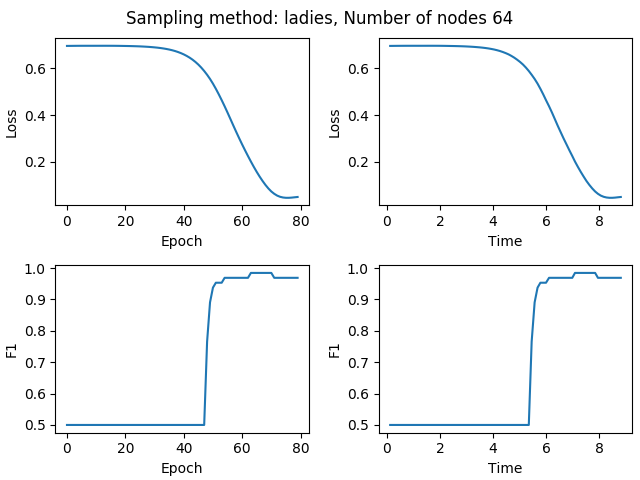
\includegraphics[scale=0.8, ]{assets/plots/ladies_64.png}
    \caption{Ladies with 64 nodes} 
\end{figure}

\begin{figure}[H]
    \centering
    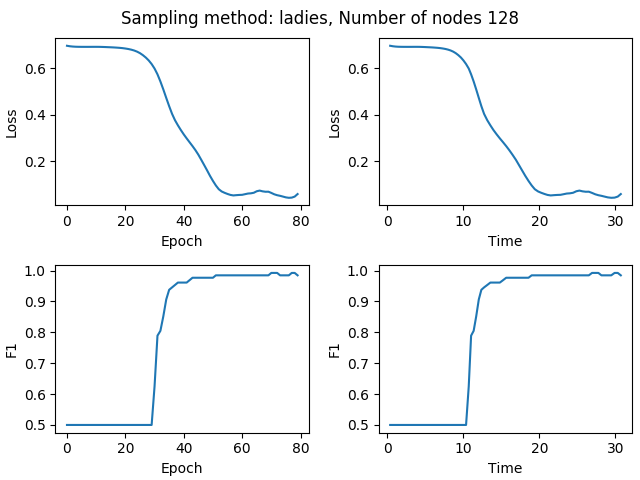
\includegraphics[scale=0.8, ]{assets/plots/ladies_128.png}
    \caption{Ladies with 128 nodes} 
\end{figure}

\begin{figure}[H]
    \centering
    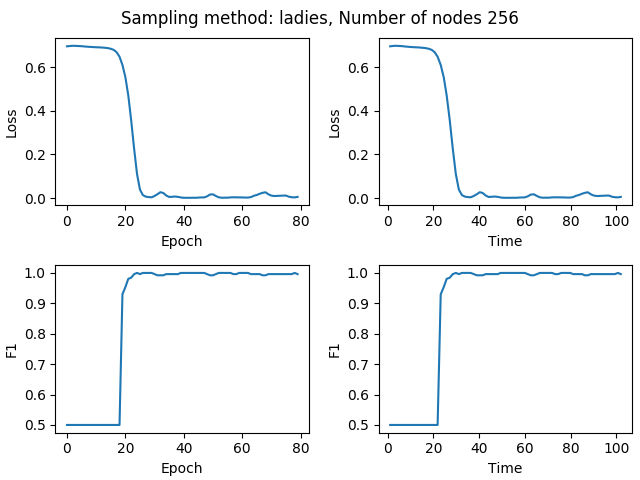
\includegraphics[scale=0.8, ]{assets/plots/ladies_256.png}
    \caption{Ladies with 256 nodes} 
\end{figure}

\begin{figure}[H]
    \centering
    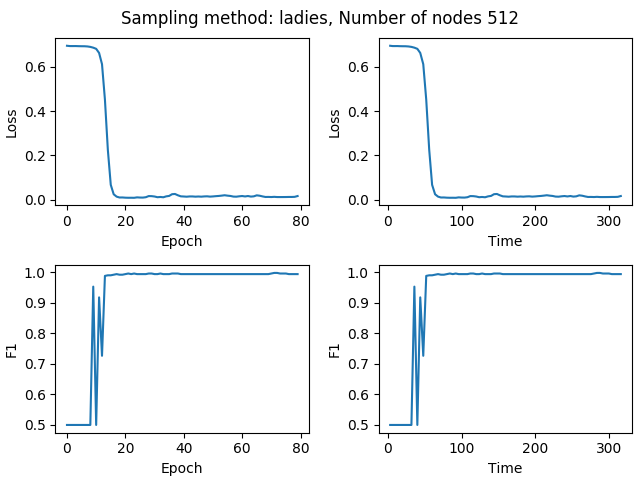
\includegraphics[scale=0.8, ]{assets/plots/ladies_512.png}
    \caption{Ladies with 512 nodes}
\end{figure}

\begin{figure}[H]
    \centering
    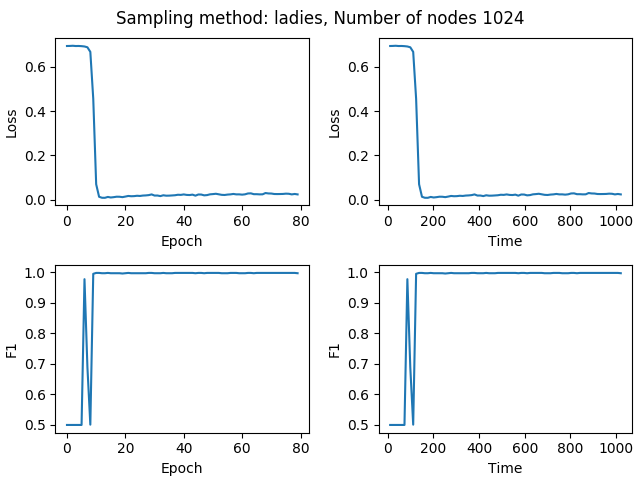
\includegraphics[scale=0.8, ]{assets/plots/ladies_1024.png}
    \caption{Ladies with 1024 nodes}
\end{figure}

\begin{figure}[H]
    \centering
    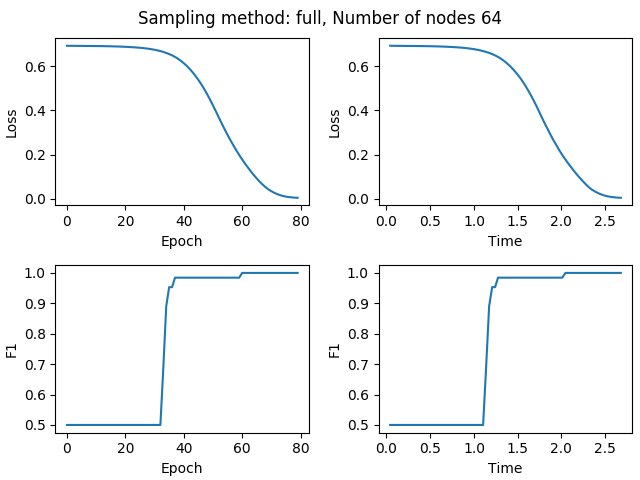
\includegraphics[scale=0.8, ]{assets/plots/full_64.png}
    \caption{Full GCN with 64 nodes}
\end{figure}

\begin{figure}[H]
    \centering
    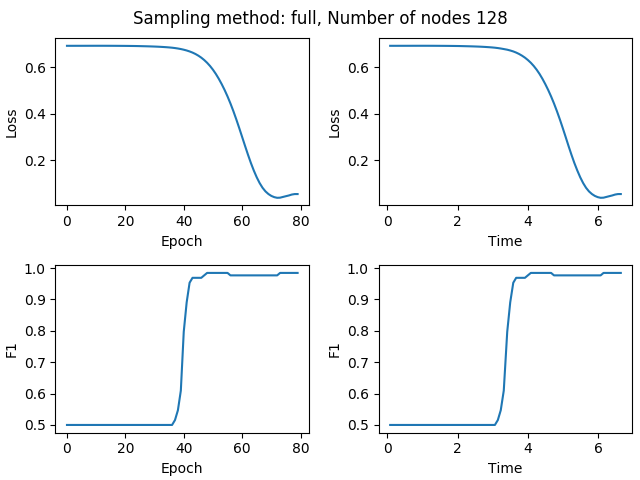
\includegraphics[scale=0.8, ]{assets/plots/full_128.png}
    \caption{Full with 128 nodes}
\end{figure}

\begin{figure}[H]
    \centering
    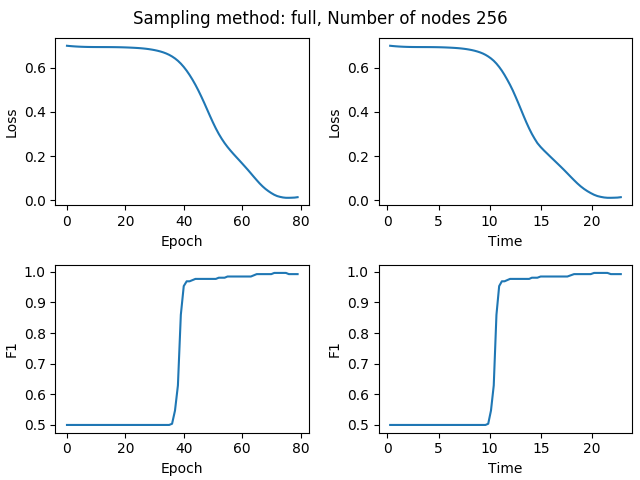
\includegraphics[scale=0.8, ]{assets/plots/full_256.png}
    \caption{Full GCN with 256 nodes}
\end{figure}

\begin{figure}[H]
    \centering
    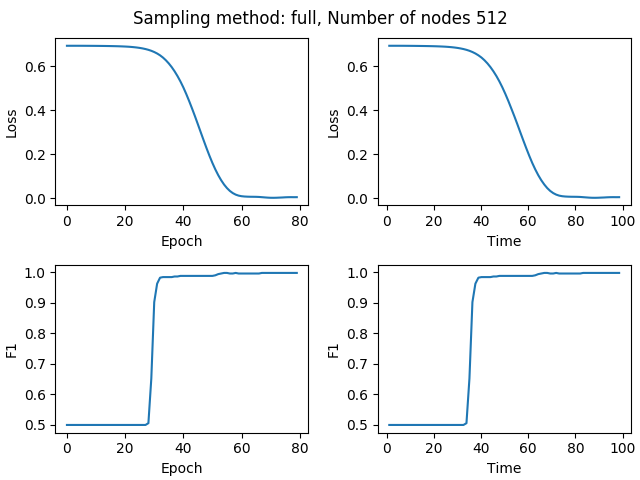
\includegraphics[scale=0.8, ]{assets/plots/full_512.png}
    \caption{Full GCN with 512 nodes}
\end{figure}

\begin{figure}[H]
    \centering
    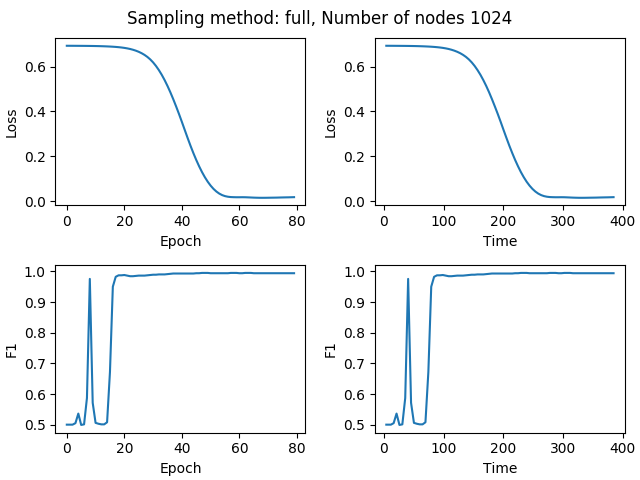
\includegraphics[scale=0.8, ]{assets/plots/full_1024.png}
    \caption{Full GCN with 1024 nodes}
\end{figure}
% \newpage
\chapter{Samples}
NOT TO BE INCLUDED IN REPORT!

Refer to this chapter for examples of figures and stuff

\section{Chapters and sections}
The order of sectioning from biggest to smallest is as such: chapter > section > subsection > subsubsection. To use simply add a backslash, for example, \textbackslash section.

\section{Figures}
\label{sample_figures}
\begin{figure}[h!]
    \centering
    
\includegraphics[scale=0.8, ]{assets/ntu_logo.png}
    \caption{Sample figure} 
    \label{fig:samp_fig}
\end{figure}

\subsection{Explanation and referencing}
As seen in figure \ref{fig:samp_fig} in section \ref{sample_figures}, this is the way to reference figures and sections. Include label to be able to reference. \textbf{If the figure does not appear exactly at the place specified, it is normal. Need to adjust figure settings such as [h!]}. Also, press \textbf{ctrl b} to \textbf{bold text}.

\section{Tables}

\begin{table}[!htbp]
\centering
\begin{tabular}{|l|l|l|}
\hline
Eddy Lim Qing Yang & U1620115B & eddy0006@e.ntu.edu.sg \\ \hline
Shawn & & @e.ntu.edu.sg \\ \hline
Leung Cheuk Yui & & cleung002@e.ntu.edu.sg \\ \hline
Joshua & & @e.ntu.edu.sg \\ \hline
& & @e.ntu.edu.sg \\ \hline
& & @e.ntu.edu.sg \\ \hline
& & @e.ntu.edu.sg \\ \hline
& & @e.ntu.edu.sg \\ \hline
\end{tabular}
\end{table}
\label{tbl:sample_table}

Table \ref{tbl:sample_table} is a sample table. Do not try to fill in the table using the latex format manually. It is more efficient to use a table generator such as in: https://www.tablesgenerator.com/.

\section{Citations}
To cite, simply use \textbackslash cite\{<articleName>\} like \cite{gunther2010neuralnet}. A bibliography list will be automatically generated.

\end{document}
